\chapter{Signal and Results}

This chapter discusses the generators used to model signal distributions and how these are parametrised for input to the statistical analysis. This is followed by the results of the data background comparison looking for any sign of new physics signal.

\section{Signal Monte Carlo}

	All signal MC is produced in the same way as the background MC and then summed with the other background predictions to arrive at the full signal prediction. Each sample also gets scaled by the same factor as the background MC from the Z peak scaling. \\


	\subsection*{Contact Interaction}

	Contact Interaction samples are generated using PYTHIA 8 \cite{Sjostrand:2007gs} with the leading order PDF MSTW2008LO \cite{Martin:2009iq}. The CI MC samples also have a K-factor applied that is derived in the same way as the DY K-factor but scaling from LO to NNLO (see section \ref{sec:MC}). A selection of $\Lambda$ values was chosen to cover the reach in new physics for all formalisms of the model (LL, LR and RR). This constituents signals for $\Lambda$ = 7, 10, 14, 20 and 28 TeV. For each of these working points parametrisations of constructive and destructive interference and LL, LR and RR models are all generated. This makes 6 parametrisations with 5 $\Lambda$ values produced for each one. Each MC sample is composed of three dilepton mass binned samples above 300 GeV in order to maintain statistics. Below 300 GeV negligible new physics is predicted and so the SM DY prediction is used below this point. 
	Because this MC sample is LO a PYTHIA 8 LO DY sample is also produced. This sample models the DY in the same way as the signal samples allowing you to subtract it from the signal samples to leave a pure new physics signal sample. This signal sample can then be added to the other background samples including the background MC DY sample (seen in section \ref{sec:MC}) to give a full signal prediction with a more consistent and higher statistics DY sample.


	\subsection*{ADD}

	The ADD samples used are produced using the SHERPA 1.4.1 \cite{1126-6708-2009-02-007} generator and NLO PDF CT10 \cite{Lai:2010vv}. Only two formalisms are produced as limits for other formalisms can be converted from the GRW one. The only formalism this is not possible for is HLZ ($n$ = 2). For these 2 formalisms 4 values of M$_{s}$ are generated of M$_{s}$ = 4.75, 4.0, 3.75 and 3.5 TeV. Again 3 dilepton mass bins are used above 300 GeV with the SM DY replacing the distribution below this. Also, like the CI samples, a specific DY only SHERPA sample is produced which is them subtracted from the signal samples so the background MC DY can be used.



\section{Signal Parametrisation}
	\label{sec:parm}

	Each formalism of the CI and ADD model is parametrised according to the form of their individual cross-sections (Eq's \ref{eq:DiffCross} and \ref{eq:ADDcs}) and as a function of their parameter of interest ($\Lambda$, M$_{s}$). The parametrisations are a prediction of number of expected events $N_{\text{exp}}$ where the parameter of interest ($\Lambda$, M$_{s}$) at $\infty$ equates to no signal and just the standard model background prediction, these can be seen in equations \ref{eq:CIparm} and \ref{eq:ADDparm}. 

	\begin{equation}
        N_{\text{exp}}(\Lambda)~=~c_{0} + \frac{c_{1}}{\Lambda^{2}} + \frac{c_{2}}{\Lambda^{4}}
        \label{eq:CIparm}
    \end{equation}

    \begin{equation}
        N_{\text{exp}}(\text{M}_{s})~=~c_{0} + \frac{c_{1}}{\text{M}_{s}^{4}} + \frac{c_{2}}{\text{M}_{s}^{8}}
        \label{eq:ADDparm}
    \end{equation}

	Here $c_{0}$ refers to the SM background prediction while $c_{1}$ and $c_{2}$ show the dependence of the scale of new physics on number of expected events. Each formalism gets parametrised in every search bin. These search bins are described at the start of chapter \ref{ch:stat} while the parametrisations can be seen in figure \ref{fig:CIparm} for every CI search bin. The full list of all of the parametrisations used can be found in appendix \ref{ap:parm}.


	\begin{figure}[h!]
	    \begin{center}
	    	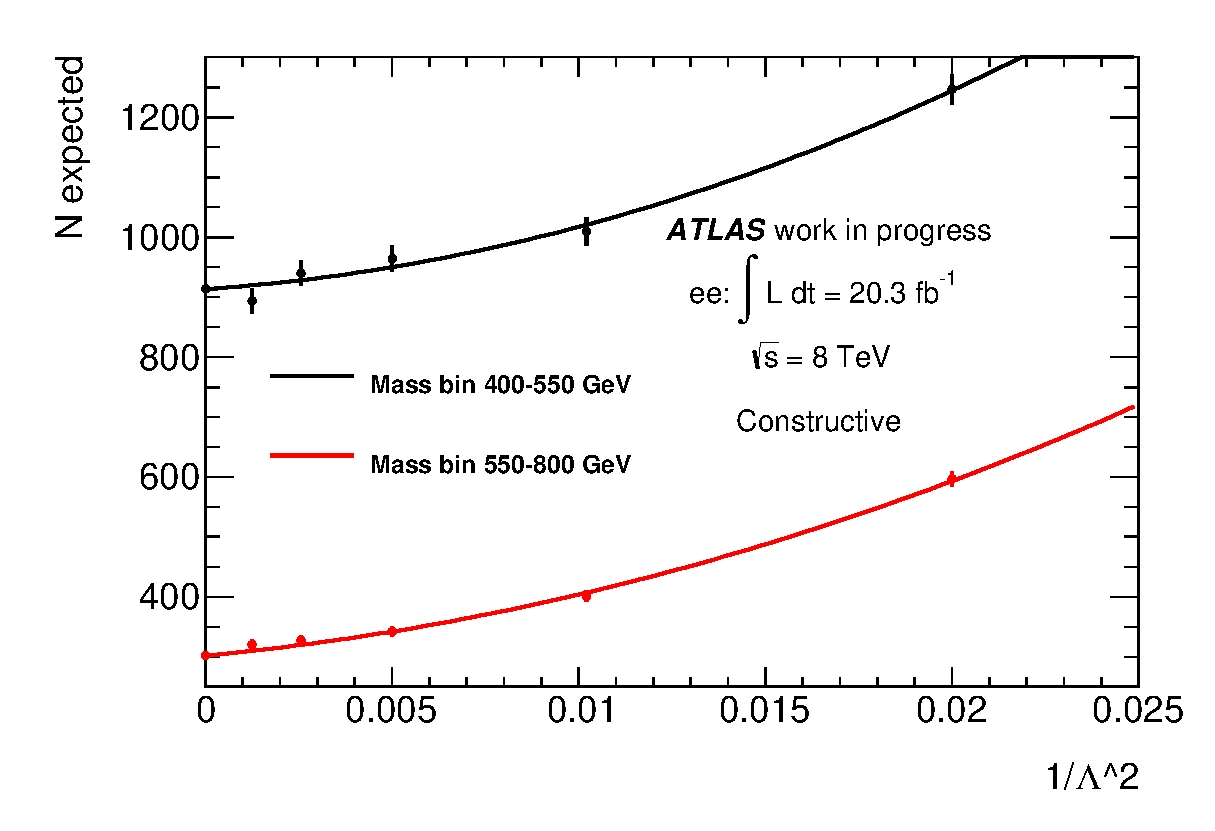
\includegraphics[width=0.49\linewidth]{images/parametrisations/NexpFits_minus_elec_lowmass.eps}
	    	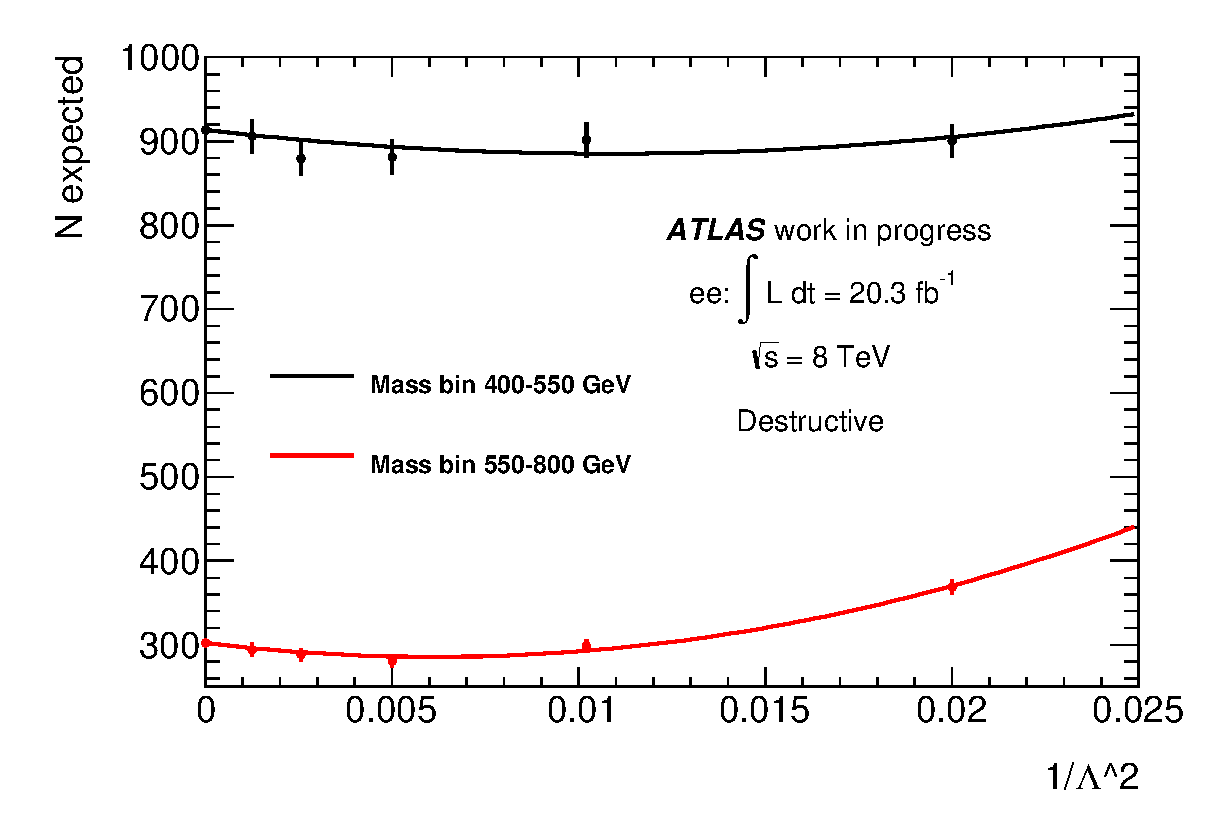
\includegraphics[width=0.49\linewidth]{images/parametrisations/NexpFits_plus_elec_lowmass.eps} \\
	    	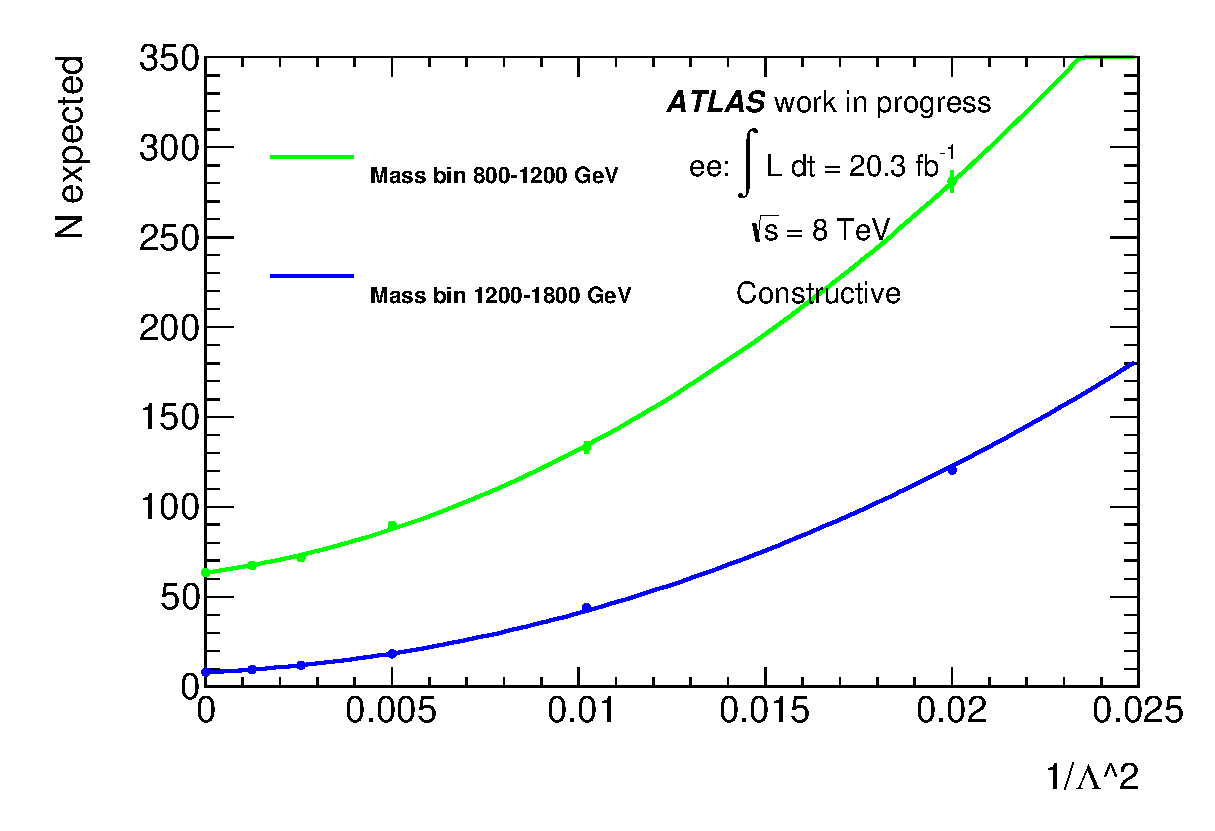
\includegraphics[width=0.49\linewidth]{images/parametrisations/NexpFits_minus_elec_midmass.eps}
	    	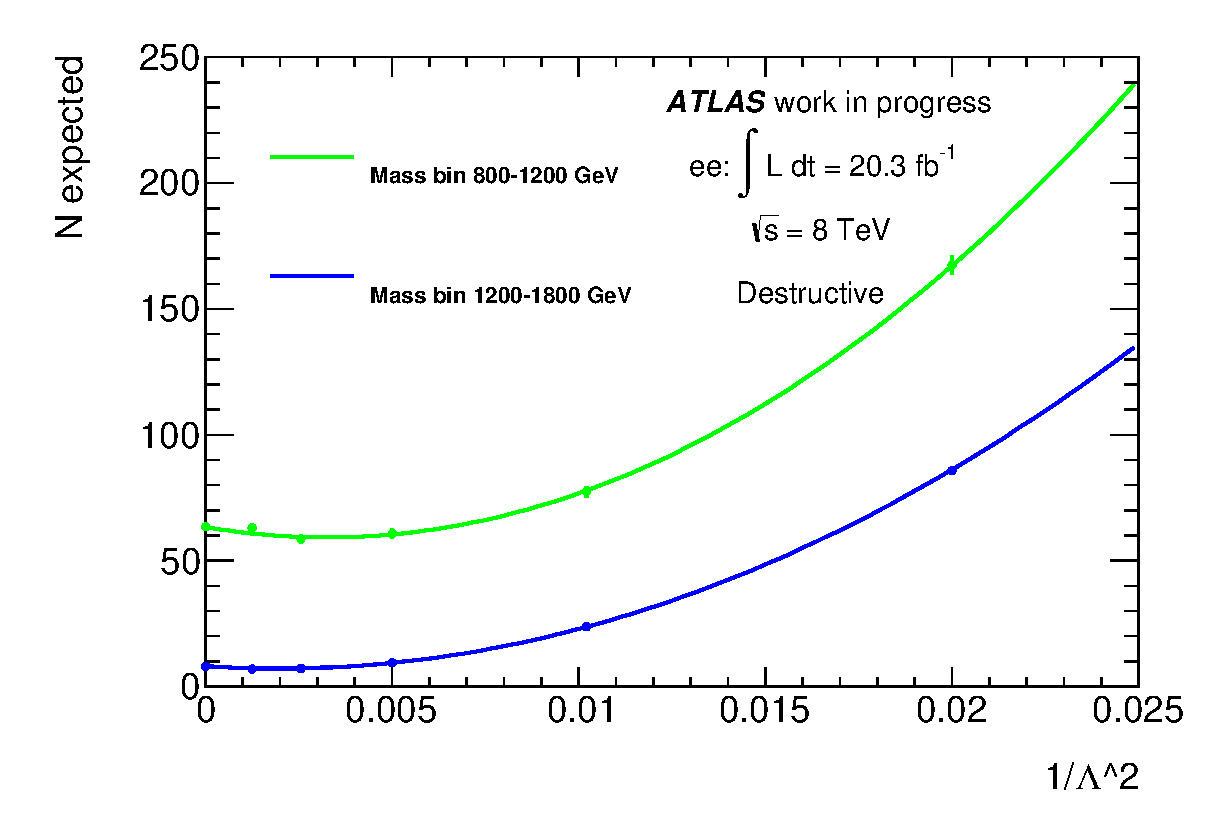
\includegraphics[width=0.49\linewidth]{images/parametrisations/NexpFits_plus_elec_midmass.eps} \\
	    	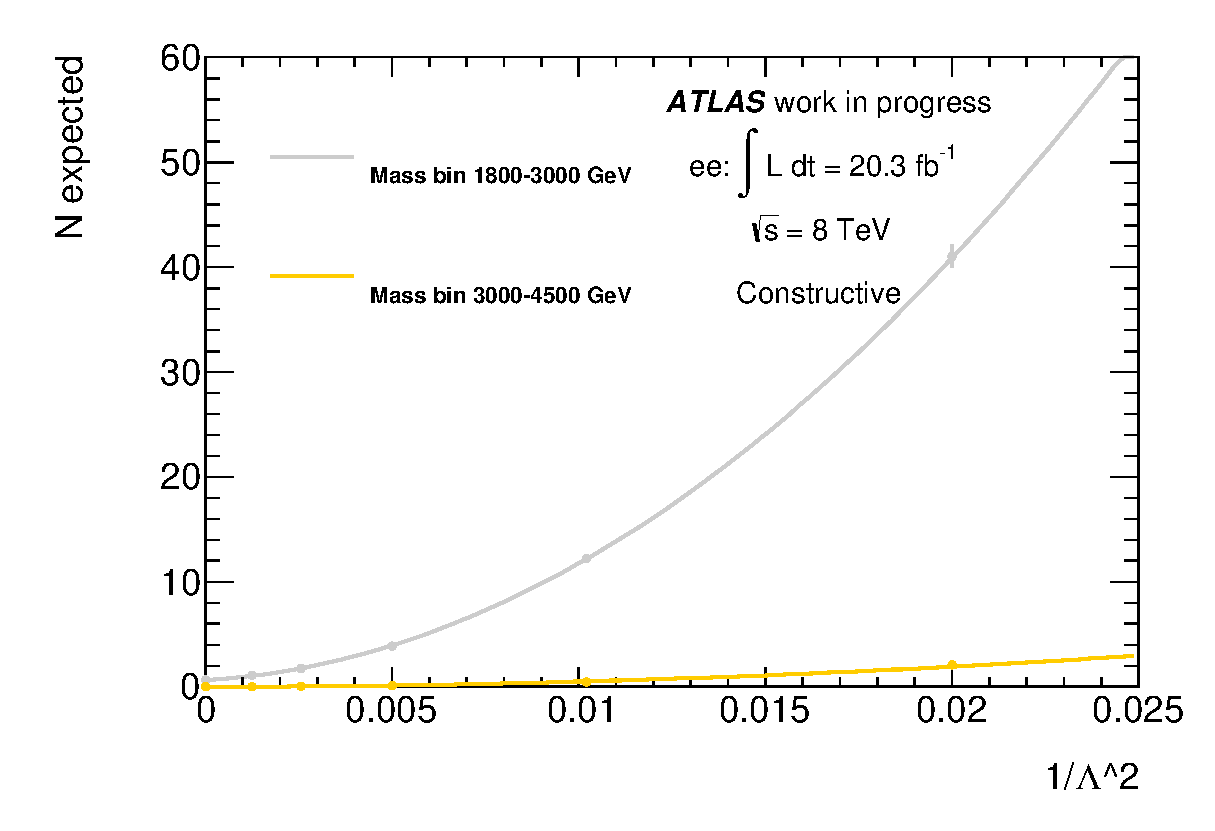
\includegraphics[width=0.49\linewidth]{images/parametrisations/NexpFits_minus_elec_himass.eps}
	    	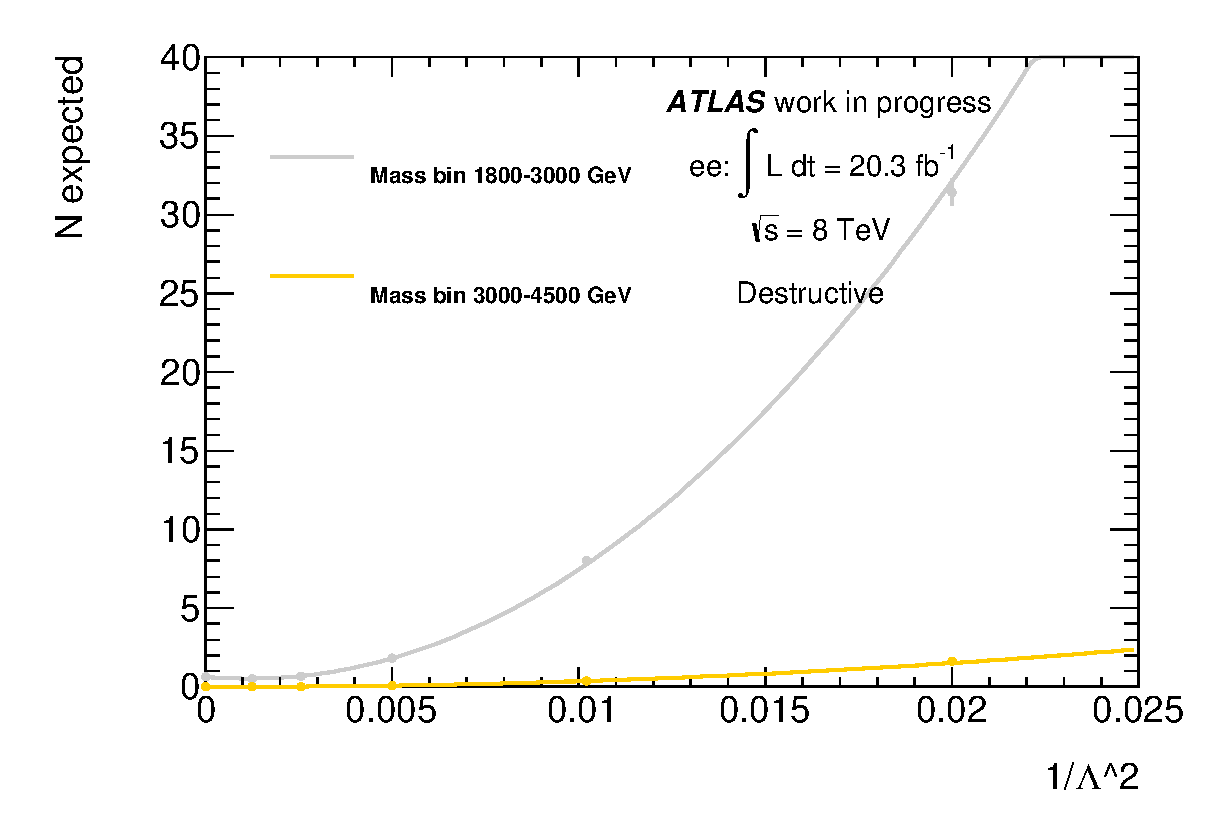
\includegraphics[width=0.49\linewidth]{images/parametrisations/NexpFits_plus_elec_himass.eps} \\
	    \end{center}
	   \caption{Parametrisations of the CI signal for number of expected events as a function of $\Lambda$ according to equation \ref{eq:CIparm} and for each CI search bin.}
	   \label{fig:CIparm}
	\end{figure}

	% \begin{figure}[h]
	%     \begin{center}
	%     	%\includegraphics[scale=0.6]{images/}
	%     \end{center}
	%    \caption{Parametrisations of the ADD signal for number of expected events as a function of M$_{s}$ according to equation \ref{eq:ADDparm} for the ADD search bin.}
	%    \label{fig:ADDparm}
	% \end{figure}


\section{Results}

	Following are full results of the event selection for observed data, predicted background and some example signal models. Figures \ref{fig:invMass_main} and \ref{fig:cosTS_main} show the distributions of the two main search variables dielectron invariant mass and $\cos{\theta^{*}}$. A comparison between data and background is given with the expected shapes of some signal models shown for comparison. Ratio's are also shown between data and background along with a band showing the size of the total systematic uncertainty as described in section \ref{sec:sys}. Figure \ref{fig:AFB_main} then shows forward backward asymmetry ($A_{FB}$) defined in equation \ref{eq:AFB}. Statistical errors on the data points are calculated using the function $\Delta A_{FB} = \sqrt{(1-A_{FB}^{2})/N}$ where $N$ is the number of events in both the forward and backwards regions. The ratio shown in figure \ref{fig:AFB_main} is the difference between data and background $A_{FB}$ values, $\Delta$, divided by the total systematic uncertainty found in that bin, $\sigma$. It can be seen that data favours the angular dependence of the SM prediction or the CI LL formalism with no divergence similar to the CI LR formalism. 
	In figure \ref{fig:control_main} control plots are seen showing electron $p_{T}$, $\eta$ and $\phi$. More results and control plots can be found in appendix \ref{ap:contol}. 
	More of all of these distributions can be seen in appendix \ref{ap:contol}.
	Lastly tables \ref{tab:CI_results0}, \ref{tab:CI_results1}, \ref{tab:CI_results2} and \ref{tab:CI_results3} show the full extracted results acceding through the search bins. Each invariant mass bin is shown as well as the forward and backwards regions within each bin where forward refers to events with $\cos{\theta^{*}}$ greater than 0 and backwards events with $\cos{\theta^{*}}$ less than 0. The expected number of events is given for each of the background as well as a selection of CI signal formalisms and the data observed. Table \ref{tab:ADD_results} shows the results for the single ADD search search bin the same as the CI tables.

	It can be seen from these results that no significant difference is seen between data observed and the background predicted. A slight discrepancy is seen between data and background in the 1200 - 1800 GeV invariant mass bin. The background predicts 10.8 events with a total systematic error of 1.6 events while only 7 events are observed in data. As seen later this doesn't signify a significant difference but has an effect on the limits set in chapter \ref{ch:stat}. 



	\begin{figure}[h]
	    \begin{center}
	    	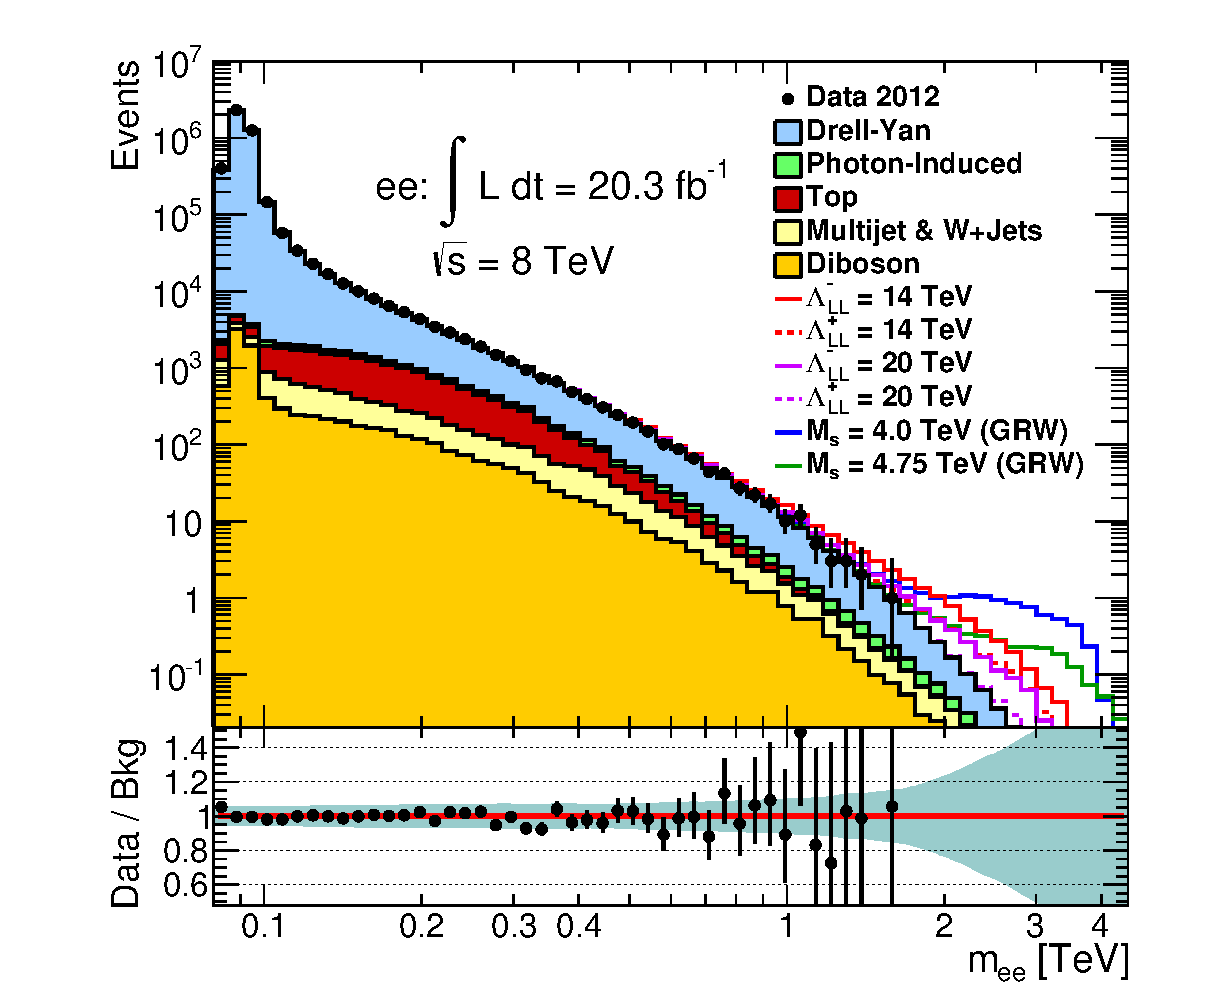
\includegraphics[width=0.8\linewidth]{images/invmass_main.eps}
	    \end{center}
	   \caption{Dielectron invariant mass comparison between data and MC with possible signal overlays of CI and ADD. Ratio between data and background included with band showing size of total background systematic. The distribution has bin width constant in $\log(M_{ee})$}
	   \label{fig:invMass_main}
	\end{figure}

	\begin{figure}[h]
	    \begin{center}
	    	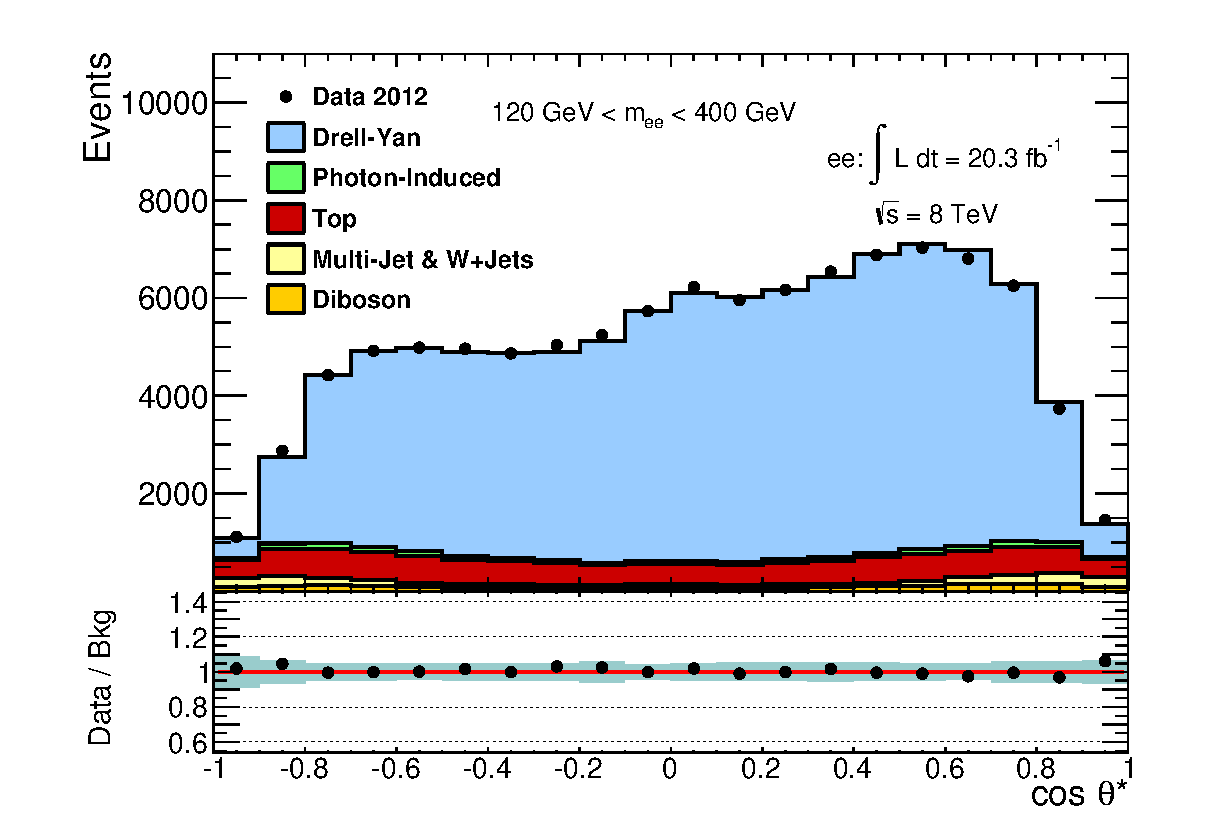
\includegraphics[width=0.9\linewidth]{images/CosThetaStar_Control_main.eps} \\
	    	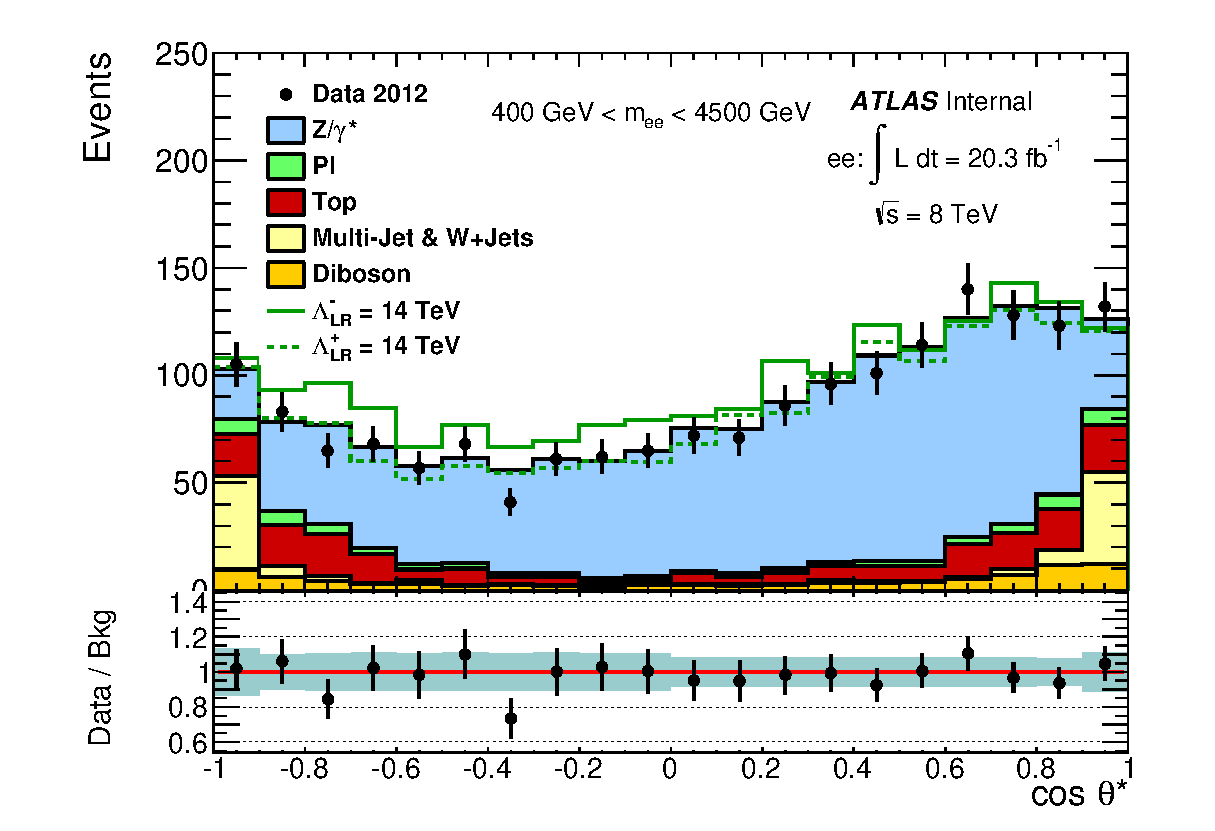
\includegraphics[width=0.9\linewidth]{images/CosThetaStar_Signal_main.eps}
	    \end{center}
	   \caption{$\cos{\theta^{*}}$ comparison between data and MC in control and signal regions with possible signal overlay of the CI LR formalism. Ratio between data and background included with band showing size of total background systematic.}
	   \label{fig:cosTS_main}
	\end{figure}

	\begin{figure}[h]
	    \begin{center}
	    	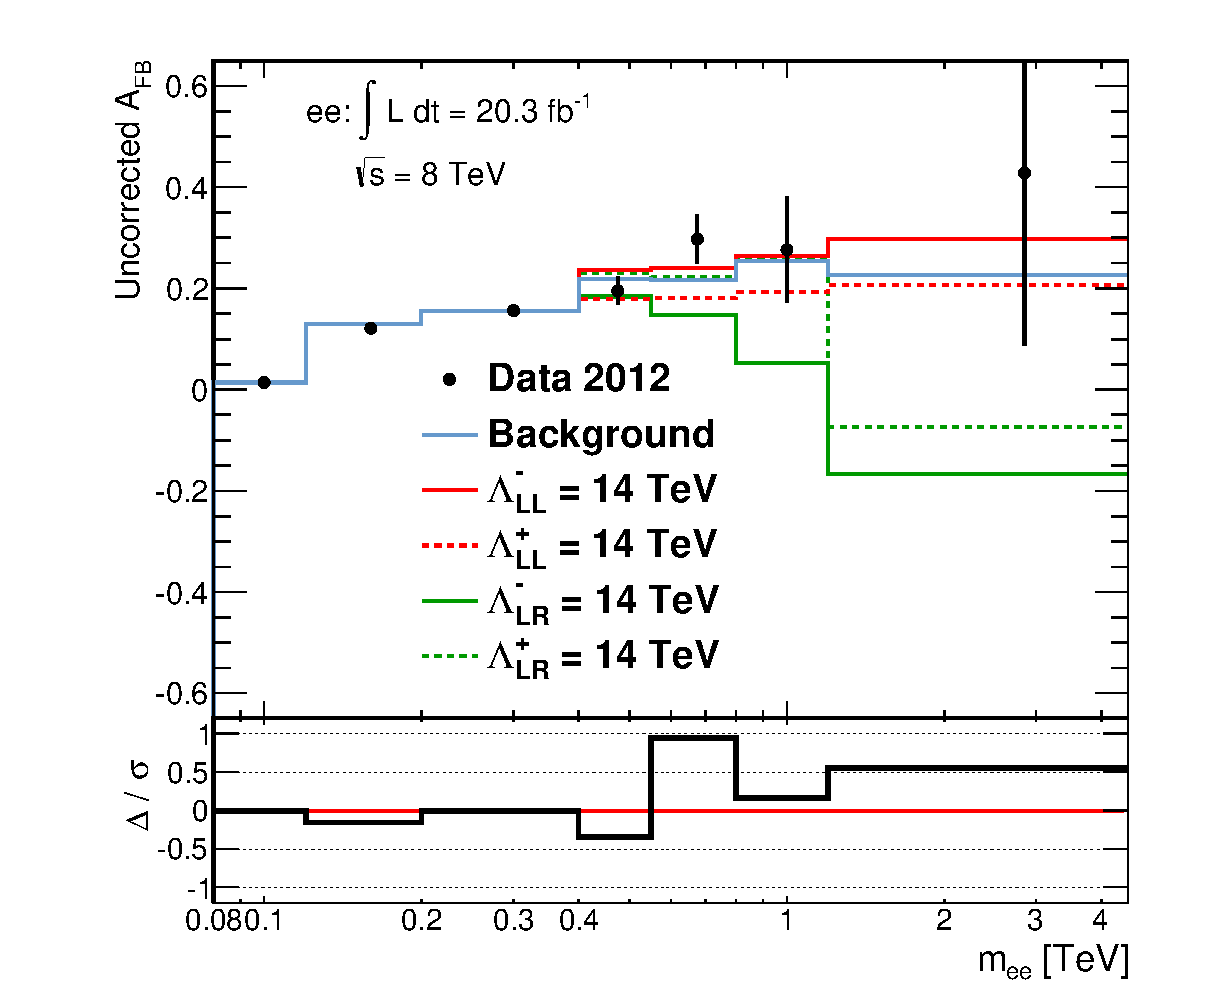
\includegraphics[width=0.8\linewidth]{images/A_fb_main.eps}
	    \end{center}
	   \caption{A$_{FB}$ comparison between data and MC with possible signal overlay of CI. Ratio shows the difference between data and background prediction divided by total background systematic.}
	   \label{fig:AFB_main}
	\end{figure}



	\begin{figure}[h]
	    \begin{center}
	    	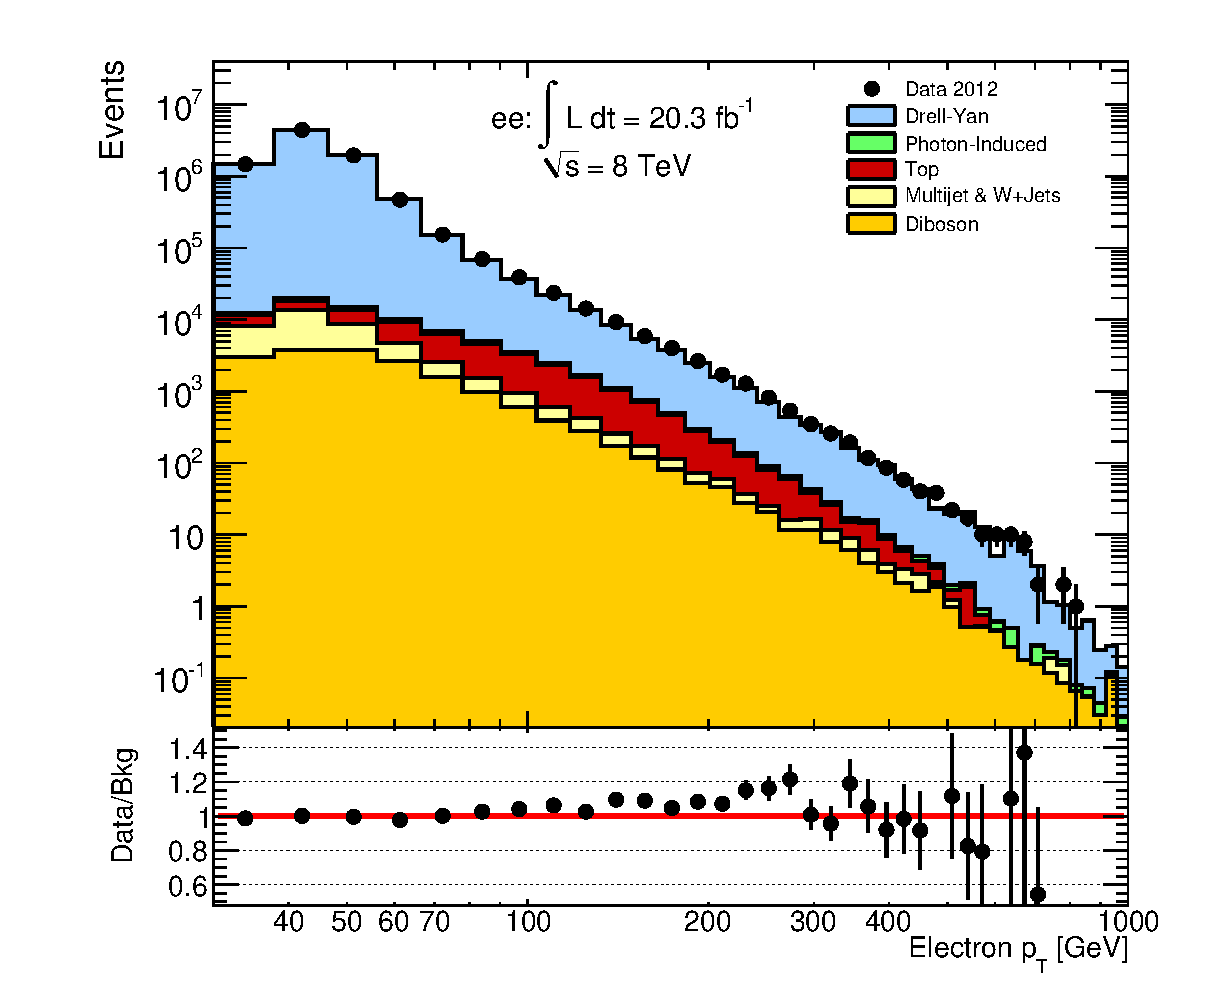
\includegraphics[width=0.8\linewidth]{images/pT_main.eps} \\
	    	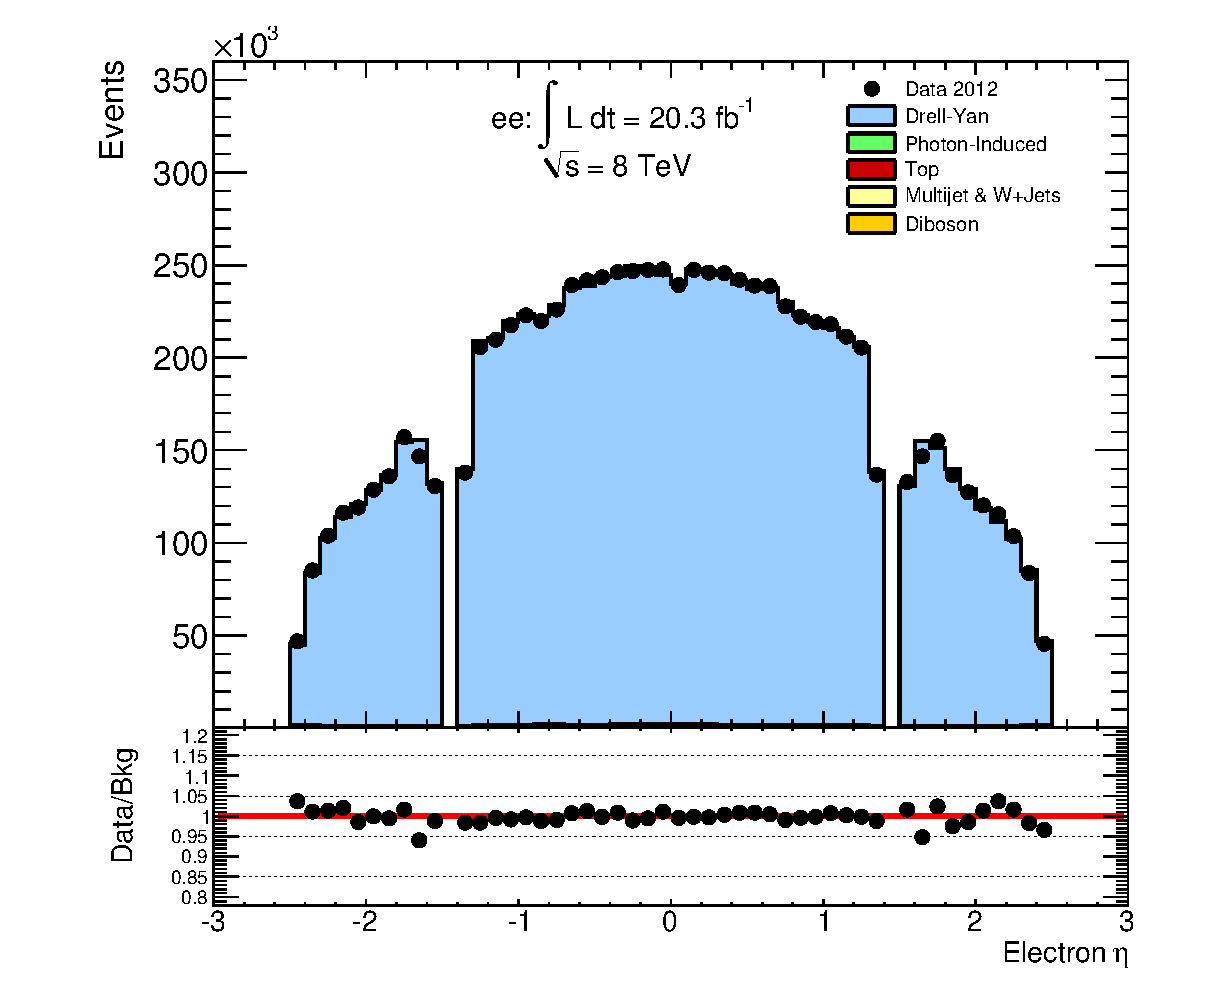
\includegraphics[width=0.49\linewidth]{images/eta_main.eps}
	    	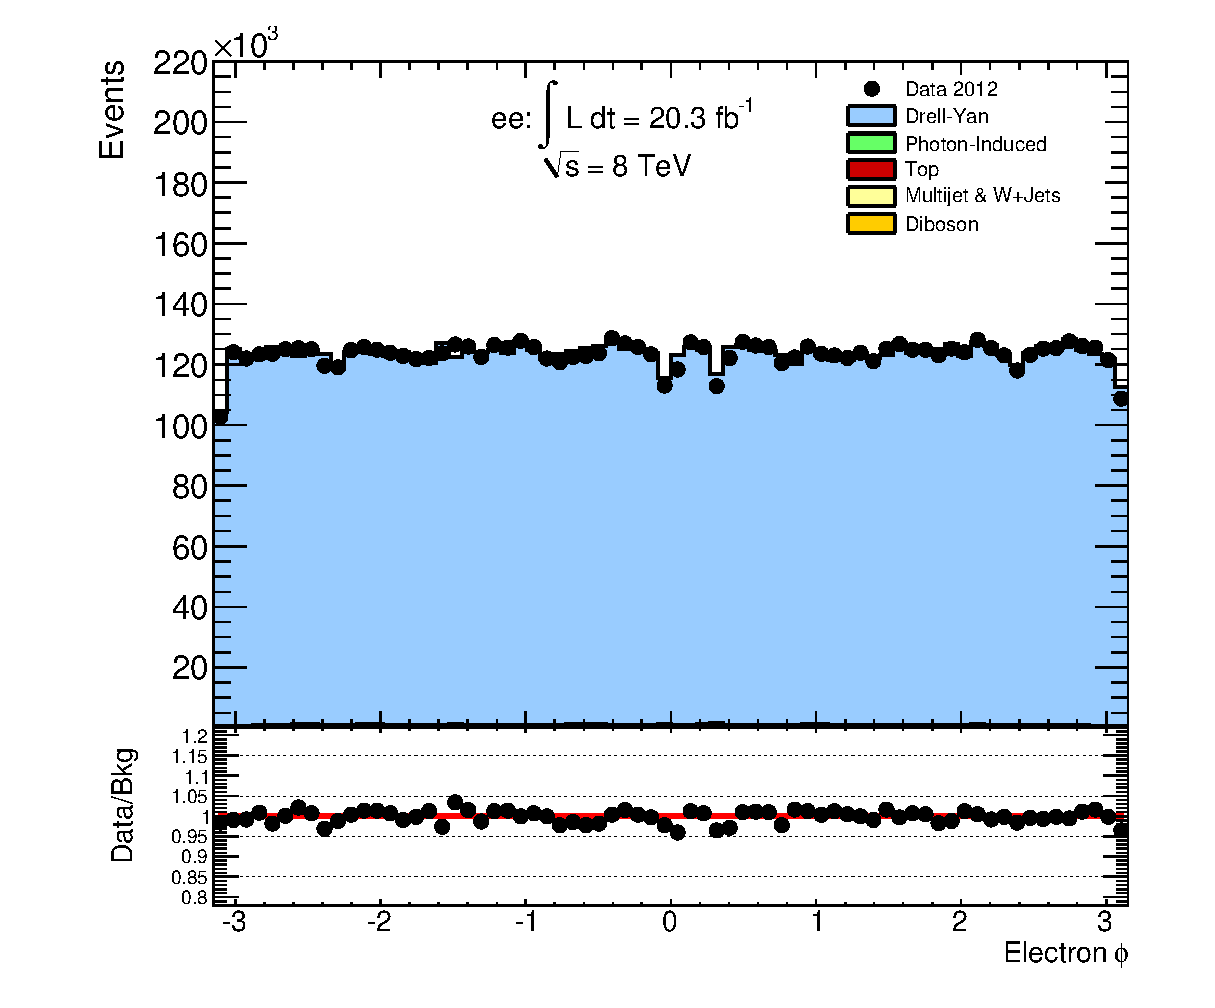
\includegraphics[width=0.49\linewidth]{images/phi_main.eps}
	    \end{center}
	   \caption{Control plots of $p_{T}$, $\eta$ and $\phi$ distributions of selected electrons.}
	   \label{fig:control_main}
	\end{figure}


	\begin {table}[h]
		\scriptsize  
		\begin{center}
		\begin{tabular}{  l | c c c | c c c  } 
			\hline
			\hline
			\multirow{3}{*}{Process} 	& \multicolumn{6}{c}{$m_{ee}$ [GeV]} \\
										& \multicolumn{3}{c}{120 - 200} & \multicolumn{3}{c}{200 - 400} \\
										\cline{2-7}
										& All & Forward & Backward & All & Forward & Backward \\
			\hline
			Drell-Yan & 72000 $\pm$ 5000 & 41500 $\pm$ 2600 & 31000 $\pm$ 2200 & 13100 $\pm$ 900 & 7900 $\pm$ 500 & 5200 $\pm$ 400 \\
			Top & 6900 $\pm$ 400 & 3480 $\pm$ 210 & 3410 $\pm$ 210 & 2840 $\pm$ 170 & 1400 $\pm$ 90 & 1440 $\pm$ 90 \\
			Multijets \& W+Jets & 1650 $\pm$ 330 & 900 $\pm$ 180 & 780 $\pm$ 160 & 670 $\pm$ 130 & 330 $\pm$ 70 & 340 $\pm$ 70 \\
			Diboson & 1330 $\pm$ 70 & 710 $\pm$ 40 & 619 $\pm$ 33 & 583 $\pm$ 31 & 331 $\pm$ 19 & 252 $\pm$ 15 \\
			Photon-Induced & 1200 $\pm$ 1200 & 600 $\pm$ 600 & 600 $\pm$ 600 & 400 $\pm$ 400 & 230 $\pm$ 230 & 220 $\pm$ 220 \\
			\hline
			Total SM & 84000 $\pm$ 5000 & 47200 $\pm$ 2800 & 36400 $\pm$ 2500 & 17600 $\pm$ 1200 & 10200 $\pm$ 600 & 7400 $\pm$ 500 \\
			\hline
			Data & 83824 & 46910 & 36914 & 17525 & 10107 & 7418 \\
			\hline
			\hline
		\end{tabular}
	  	\caption{Table comparing background prediction to data. Binning covering the control region. Total systematic error is included on each number. See section \ref{sec:sys} for details of systematics.}
	  	\label{tab:CI_results0}
	  	\end{center}
	\end {table}

	\begin {table}[h]
		\scriptsize  
		\begin{center}
		\begin{tabular}{  l | c c c | c c c  } 
			\hline
			\hline
			\multirow{3}{*}{Process} 	& \multicolumn{6}{c}{$m_{ee}$ [GeV]} \\
										& \multicolumn{3}{c}{400 - 550} & \multicolumn{3}{c}{550 - 800} \\
										\cline{2-7}
										& All & Forward & Backward & All & Forward & Backward \\
			\hline
			Drell-Yan & 910 $\pm$ 70 & 580 $\pm$ 40 & 333 $\pm$ 32 & 302 $\pm$ 25 & 193 $\pm$ 13 & 109 $\pm$ 12 \\
			Top & 153 $\pm$ 13 & 87 $\pm$ 8 & 72 $\pm$ 7 & 35.2 $\pm$ 2.7 & 18.2 $\pm$ 1.6 & 17.5 $\pm$ 1.6 \\
			Multijets \& W+Jets & 88 $\pm$ 18 & 43 $\pm$ 9 & 45 $\pm$ 9 & 27 $\pm$ 6 & 13.0 $\pm$ 3.0 & 13.0 $\pm$ 3.1 \\
			Diboson & 62.2 $\pm$ 3.5 & 36.0 $\pm$ 2.2 & 26.2 $\pm$ 1.7 & 22.3 $\pm$ 1.3 & 13.8 $\pm$ 0.9 & 8.5 $\pm$ 0.7 \\
			Photon-Induced & 40 $\pm$ 40 & 22 $\pm$ 22 & 22 $\pm$ 22 & 17 $\pm$ 17 & 8 $\pm$ 8 & 8 $\pm$ 8 \\
			\hline
			Total SM & 1260 $\pm$ 100 & 770 $\pm$ 50 & 500 $\pm$ 50 & 404 $\pm$ 35 & 247 $\pm$ 18 & 156 $\pm$ 17 \\
			\hline
			Data & 1262 & 754 & 508 & 388 & 251 & 137 \\
			\hline
			SM+CI($\Lambda^{-14}_{LL}$) & 1310 $\pm$ 110 & 810 $\pm$ 60 & 510 $\pm$ 50 & 440 $\pm$ 40 & 276 $\pm$ 22 & 167 $\pm$ 18 \\
			SM+CI($\Lambda^{-20}_{LL}$) & 1290 $\pm$ 110 & 780 $\pm$ 60 & 510 $\pm$ 50 & 430 $\pm$ 40 & 271 $\pm$ 22 & 157 $\pm$ 18 \\
			SM+CI($\Lambda^{-14}_{LR}$) & 1340 $\pm$ 110 & 790 $\pm$ 60 & 550 $\pm$ 50 & 460 $\pm$ 40 & 266 $\pm$ 22 & 195 $\pm$ 19 \\
			SM+CI($\Lambda^{-20}_{LR}$) & 1290 $\pm$ 110 & 780 $\pm$ 60 & 510 $\pm$ 50 & 420 $\pm$ 40 & 249 $\pm$ 21 & 174 $\pm$ 19 \\
			SM+CI($\Lambda^{-14}_{RR}$) & 1310 $\pm$ 110 & 810 $\pm$ 60 & 510 $\pm$ 50 & 440 $\pm$ 40 & 276 $\pm$ 22 & 167 $\pm$ 18 \\
			SM+CI($\Lambda^{-20}_{RR}$) & 1290 $\pm$ 110 & 780 $\pm$ 60 & 510 $\pm$ 50 & 430 $\pm$ 40 & 271 $\pm$ 22 & 157 $\pm$ 18 \\
			\hline
			SM+CI($\Lambda^{+14}_{LL}$) & 1230 $\pm$ 110 & 730 $\pm$ 60 & 510 $\pm$ 50 & 380 $\pm$ 40 & 227 $\pm$ 21 & 155 $\pm$ 18 \\
			SM+CI($\Lambda^{+20}_{LL}$) & 1230 $\pm$ 110 & 740 $\pm$ 60 & 490 $\pm$ 50 & 390 $\pm$ 40 & 234 $\pm$ 21 & 156 $\pm$ 18 \\
			SM+CI($\Lambda^{+14}_{LR}$) & 1200 $\pm$ 110 & 740 $\pm$ 60 & 470 $\pm$ 50 & 400 $\pm$ 40 & 247 $\pm$ 21 & 154 $\pm$ 18 \\
			SM+CI($\Lambda^{+20}_{LR}$) & 1210 $\pm$ 110 & 740 $\pm$ 60 & 470 $\pm$ 50 & 390 $\pm$ 40 & 238 $\pm$ 21 & 150 $\pm$ 18 \\
			SM+CI($\Lambda^{+14}_{RR}$) & 1230 $\pm$ 110 & 730 $\pm$ 60 & 510 $\pm$ 50 & 380 $\pm$ 40 & 227 $\pm$ 21 & 155 $\pm$ 18 \\
			SM+CI($\Lambda^{+20}_{RR}$) & 1230 $\pm$ 110 & 740 $\pm$ 60 & 490 $\pm$ 50 & 390 $\pm$ 40 & 234 $\pm$ 21 & 156 $\pm$ 18 \\
			\hline
			\hline
		\end{tabular}
	  	\caption{Table comparing background prediction to data with prediction of several CI signal models. Binning used is the same as used for statistical analysis of CI model with search bins 1 and 2 shown here. Total systematic error is included on each number. See section \ref{sec:sys} for details of systematics.}
	  	\label{tab:CI_results1}
	  	\end{center}
	\end {table}

	\begin {table}[h]
		\scriptsize 
		\begin{center}
		\begin{tabular}{  l | c c c | c c c  }	
			\hline
			\hline
			\multirow{3}{*}{Process} 	& \multicolumn{6}{c}{$m_{ee}$ [GeV]} \\
										& \multicolumn{3}{c}{800 - 1200} & \multicolumn{3}{c}{1200 - 1800} \\
										\cline{2-7}
										& All & Forward & Backward & All & Forward & Backward \\
			\hline
			Drell-Yan & 63 $\pm$ 6 & 41.4 $\pm$ 3.4 & 22.1 $\pm$ 2.9 & 8.2 $\pm$ 1.2 & 5.3 $\pm$ 0.6 & 2.9 $\pm$ 0.6 \\
			Top & 3.06 $\pm$ 0.18 & 1.58 $\pm$ 0.10 & 1.45 $\pm$ 0.09 & 0.140 $\pm$ 0.008 & 0.073 $\pm$ 0.004 & 0.065 $\pm$ 0.004 \\
			Multijets \& W+Jets & 5.8 $\pm$ 1.5 & 2.6 $\pm$ 0.9 & 2.5 $\pm$ 0.8 & 0.87 $\pm$ 0.32 & 0.35 $\pm$ 0.16 & 0.32 $\pm$ 0.24 \\
			Diboson & 5.4 $\pm$ 0.4 & 3.41 $\pm$ 0.28 & 2.02 $\pm$ 0.17 & 0.83 $\pm$ 0.05 & 0.542 $\pm$ 0.035 & 0.287 $\pm$ 0.016 \\
			Photon-Induced & 4 $\pm$ 4 & 2.2 $\pm$ 2.2 & 2.1 $\pm$ 2.1 & 0.7 $\pm$ 0.7 & 0.34 $\pm$ 0.34 & 0.4 $\pm$ 0.4 \\
			\hline
			Total SM & 82 $\pm$ 9 & 51 $\pm$ 5 & 30 $\pm$ 4 & 10.8 $\pm$ 1.6 & 6.6 $\pm$ 0.7 & 4.0 $\pm$ 0.8 \\
			\hline
			Data & 84 & 53 & 31 & 7 & 5 & 2 \\
			\hline
			SM+CI($\Lambda^{-14}_{LL}$) & 108 $\pm$ 10 & 68 $\pm$ 6 & 39 $\pm$ 5 & 20.9 $\pm$ 1.9 & 13.5 $\pm$ 1.0 & 7.2 $\pm$ 0.9 \\
			SM+CI($\Lambda^{-20}_{LL}$) & 90 $\pm$ 10 & 58 $\pm$ 5 & 32 $\pm$ 4 & 14.4 $\pm$ 1.7 & 9.2 $\pm$ 0.9 & 5.0 $\pm$ 0.8 \\
			SM+CI($\Lambda^{-14}_{LR}$) & 118 $\pm$ 10 & 62 $\pm$ 6 & 56 $\pm$ 5 & 26.3 $\pm$ 2.1 & 11.3 $\pm$ 1.0 & 14.8 $\pm$ 1.1 \\
			SM+CI($\Lambda^{-20}_{LR}$) & 98 $\pm$ 10 & 57 $\pm$ 5 & 41 $\pm$ 5 & 15.7 $\pm$ 1.7 & 8.3 $\pm$ 0.9 & 7.2 $\pm$ 0.9 \\
			SM+CI($\Lambda^{-14}_{RR}$) & 108 $\pm$ 10 & 68 $\pm$ 6 & 40 $\pm$ 5 & 20.8 $\pm$ 1.9 & 13.6 $\pm$ 1.0 & 6.9 $\pm$ 0.9 \\
			SM+CI($\Lambda^{-20}_{RR}$) & 91 $\pm$ 10 & 58 $\pm$ 5 & 32 $\pm$ 4 & 14.3 $\pm$ 1.7 & 9.1 $\pm$ 0.9 & 5.0 $\pm$ 0.8 \\
			\hline
			SM+CI($\Lambda^{+14}_{LL}$) & 79 $\pm$ 9 & 47 $\pm$ 5 & 32 $\pm$ 4 & 12.2 $\pm$ 1.7 & 7.3 $\pm$ 0.8 & 4.7 $\pm$ 0.8 \\
			SM+CI($\Lambda^{+20}_{LL}$) & 77 $\pm$ 9 & 48 $\pm$ 5 & 29 $\pm$ 4 & 10.0 $\pm$ 1.6 & 6.1 $\pm$ 0.8 & 3.7 $\pm$ 0.8 \\
			SM+CI($\Lambda^{+14}_{LR}$) & 88 $\pm$ 10 & 55 $\pm$ 5 & 32 $\pm$ 4 & 18.9 $\pm$ 1.8 & 9.2 $\pm$ 0.9 & 9.5 $\pm$ 0.9 \\
			SM+CI($\Lambda^{+20}_{LR}$) & 81 $\pm$ 9 & 52 $\pm$ 5 & 29 $\pm$ 4 & 11.5 $\pm$ 1.6 & 6.8 $\pm$ 0.8 & 4.5 $\pm$ 0.8 \\
			SM+CI($\Lambda^{+14}_{RR}$) & 79 $\pm$ 9 & 47 $\pm$ 5 & 32 $\pm$ 4 & 12.1 $\pm$ 1.7 & 7.3 $\pm$ 0.8 & 4.6 $\pm$ 0.8 \\
			SM+CI($\Lambda^{+20}_{RR}$) & 77 $\pm$ 9 & 48 $\pm$ 5 & 29 $\pm$ 4 & 10.2 $\pm$ 1.6 & 6.3 $\pm$ 0.8 & 3.8 $\pm$ 0.8 \\
			\hline
			\hline
		\end{tabular}
	  	\caption{Table comparing background prediction to data with prediction of several CI signal models. Binning used is the same as used for statistical analysis of CI model with search bins 3 and 4 shown here. Total systematic error is included on each number. See section \ref{sec:sys} for details of systematics.}
	  	\label{tab:CI_results2}
	  	\end{center}
	\end {table}



	\begin {table}[h]
		\scriptsize 
		\begin{center}
		\begin{tabular}{  l | c c c | c c c  }
			\hline
			\hline
			\multirow{3}{*}{Process} 	& \multicolumn{6}{c}{$m_{ee}$ [GeV]} \\
										& \multicolumn{3}{c}{1800 - 3000} & \multicolumn{3}{c}{3000 - 4500} \\
										\cline{2-7}
										& All & Forward & Backward & All & Forward & Backward \\
			\hline
			Drell-Yan & 0.64 $\pm$ 0.17 & 0.41 $\pm$ 0.09 & 0.23 $\pm$ 0.08 & 0.006 $\pm$ 0.004 & 0.0039 $\pm$ 0.0021 & 0.0022 $\pm$ 0.0018 \\
			Top & $<$ 0.004   & $<$ 0.002   & $<$ 0.002   & $<$ 0.001   & $<$ 0.001   & $<$ 0.001   \\
			Multijets \& W+Jets & 0.11 $\pm$ 0.04 & 0.040 $\pm$ 0.020 & 0.033 $\pm$ 0.027 & 0.0058 $\pm$ 0.0012 & $<$ 0.002   & $<$ 0.001   \\
			Diboson & 0.075 $\pm$ 0.006 & 0.053 $\pm$ 0.004 & 0.0224 $\pm$ 0.0026 & $<$ 0.001   & $<$ 0.001   & $<$ 0.001   \\
			Photon-Induced & 0.08 $\pm$ 0.08 & 0.04 $\pm$ 0.04 & 0.04 $\pm$ 0.04 & 0.0016 $\pm$ 0.0016 & $<$ 0.002   & $<$ 0.002   \\
			\hline
			Total SM & 0.91 $\pm$ 0.21 & 0.55 $\pm$ 0.10 & 0.33 $\pm$ 0.10 & 0.014 $\pm$ 0.005 & 0.0065 $\pm$ 0.0026 & 0.0042 $\pm$ 0.0022 \\
			\hline
			Data & 0 & 0 & 0 & 0 & 0 & 0 \\
			\hline
			SM+CI($\Lambda^{-14}_{LL}$) & 4.2 $\pm$ 0.4 & 2.75 $\pm$ 0.23 & 1.38 $\pm$ 0.15 & 0.141 $\pm$ 0.028 & 0.080 $\pm$ 0.020 & 0.058 $\pm$ 0.016 \\
			SM+CI($\Lambda^{-20}_{LL}$) & 2.01 $\pm$ 0.25 & 1.26 $\pm$ 0.14 & 0.72 $\pm$ 0.12 & 0.045 $\pm$ 0.012 & 0.021 $\pm$ 0.007 & 0.022 $\pm$ 0.007 \\
			SM+CI($\Lambda^{-14}_{LR}$) & 6.0 $\pm$ 0.5 & 2.31 $\pm$ 0.21 & 3.69 $\pm$ 0.30 & 0.28 $\pm$ 0.05 & 0.127 $\pm$ 0.030 & 0.146 $\pm$ 0.032 \\
			SM+CI($\Lambda^{-20}_{LR}$) & 2.58 $\pm$ 0.28 & 1.01 $\pm$ 0.13 & 1.54 $\pm$ 0.16 & 0.078 $\pm$ 0.018 & 0.036 $\pm$ 0.011 & 0.039 $\pm$ 0.012 \\
			SM+CI($\Lambda^{-14}_{RR}$) & 3.78 $\pm$ 0.34 & 2.51 $\pm$ 0.22 & 1.23 $\pm$ 0.15 & 0.23 $\pm$ 0.04 & 0.155 $\pm$ 0.031 & 0.069 $\pm$ 0.018 \\
			SM+CI($\Lambda^{-20}_{RR}$) & 1.86 $\pm$ 0.24 & 1.11 $\pm$ 0.13 & 0.71 $\pm$ 0.12 & 0.072 $\pm$ 0.015 & 0.047 $\pm$ 0.011 & 0.022 $\pm$ 0.008 \\
			\hline
			SM+CI($\Lambda^{+14}_{LL}$) & 2.08 $\pm$ 0.25 & 1.30 $\pm$ 0.14 & 0.75 $\pm$ 0.12 & 0.075 $\pm$ 0.015 & 0.050 $\pm$ 0.012 & 0.023 $\pm$ 0.007 \\
			SM+CI($\Lambda^{+20}_{LL}$) & 0.95 $\pm$ 0.22 & 0.55 $\pm$ 0.11 & 0.36 $\pm$ 0.11 & 0.029 $\pm$ 0.008 & 0.019 $\pm$ 0.006 & 0.0073 $\pm$ 0.0034 \\
			SM+CI($\Lambda^{+14}_{LR}$) & 4.2 $\pm$ 0.4 & 1.60 $\pm$ 0.16 & 2.51 $\pm$ 0.22 & 0.191 $\pm$ 0.034 & 0.081 $\pm$ 0.020 & 0.107 $\pm$ 0.023 \\
			SM+CI($\Lambda^{+20}_{LR}$) & 1.65 $\pm$ 0.24 & 0.82 $\pm$ 0.12 & 0.79 $\pm$ 0.12 & 0.058 $\pm$ 0.013 & 0.017 $\pm$ 0.006 & 0.039 $\pm$ 0.010 \\
			SM+CI($\Lambda^{+14}_{RR}$) & 2.26 $\pm$ 0.26 & 1.44 $\pm$ 0.15 & 0.78 $\pm$ 0.12 & 0.098 $\pm$ 0.018 & 0.057 $\pm$ 0.012 & 0.038 $\pm$ 0.010 \\
			SM+CI($\Lambda^{+20}_{RR}$) & 1.06 $\pm$ 0.22 & 0.65 $\pm$ 0.11 & 0.37 $\pm$ 0.11 & 0.036 $\pm$ 0.009 & 0.028 $\pm$ 0.008 & 0.0044 $\pm$ 0.0029 \\
			\hline
	    	\hline
	  	\end{tabular}
	  	\caption{Table comparing background prediction to data with prediction of several CI signal models. Binning used is the same as used for statistical analysis of CI model with search bins 5 and 6 shown here. Total systematic error is included on each number. See section \ref{sec:sys} for details of systematics.}
	  	\label{tab:CI_results3}
	  	\end{center}
	\end {table}






	\begin {table}[h]
		\begin{center}
		\begin{tabular}{  l | c } 
			\hline
			\hline
			Process & 1900 $\le$ $m_{ee}$ $\le$ 4500 GeV \\
			\hline
			Drell-Yan & 0.435 $\pm$ 0.002 \\
			Top & 0.003$\pm$ 0.000 \\
			Multi-Jet & 0.062 $\pm$ 0.012 \\
			Diboson & 0.053 $\pm$ 0.004 \\
			Photon-Induced & 0.058 $\pm$ 0.001 \\
			\hline
			Total SM & 0.611 $\pm$ 0.129 \\
			\hline
			Data & 0 \\ 
			\hline
			SM+ADD ($M_{S}$ = 3.50~TeV)& 21.637 $\pm$  2.144 \\
			SM+ADD ($M_{S}$ = 3.75~TeV)& 13.171 $\pm$  1.295 \\
			SM+ADD ($M_{S}$ = 4.00~TeV)& 8.436 $\pm$  0.821 \\
			SM+ADD ($M_{S}$ = 4.75~TeV)& 2.952 $\pm$  0.282 \\
	    	\hline
	    	\hline
	  	\end{tabular}
	  	\caption{Table comparing background prediction to data with prediction of several ADD signal models. One bin used the same in the statistical analysis of ADD. Total systematic error is included on each number. See section \ref{sec:sys} for details of systematics.}
	  	\label{tab:ADD_results}
	  	\end{center}
	\end {table}









